In this section, we report the results of the proposed framework for different configurations of the illustrative example in \sref{illustrative-example}.
All the experiments are conducted on a GNU/Linux machine with Intel Core i7 2.66~GHz and 8~GB of RAM.

Now we shall describe the default configuration of our experimental setup, which, in the following subsections, will be adjusted according to the purpose of each particular experiment.
We consider a 45-nanometer technological process.
The effective channel length is assumed to deviate by $5\%$ from the nominal value of 45~nm where the global and local variations are equally weighted \cite{juan2011, juan2012}.
Correlation matrices are computed according to \eref{correlation-function} where the length-scale parameters $\ell_\SE$ and $\ell_\OU$ are set to half the size of the die.
In the model order reduction technique (see \sref{ie-uncertain-parameters}), the threshold parameter is set to $0.99$ preserving $99\%$ of the variance of the data.
Dynamic power profiles involved in the experiments are based on simulations of randomly generated, \via\ TGFF (v3.5) \cite{dick1998}, applications defined as directed acyclic task graphs.
The floorplans of the platforms are constructed in such a way that the processing elements form regular grids.\footnote{The task graphs of the applications, floorplans of the platforms, configuration of HotSpot, which is used to construct the thermal RC circuits, are available online at \cite{sources}.}
Time steps of power and temperature traces are set to one millisecond (see \sref{problem-formulation}).
To assess the performance of our framework, we employ a Monte Carlo (MC) sampling technique.
For each sample, \ie, for each outcome of the uncertain parameters, the MC approach solves the initial problem in \eref{fourier-system} numerically using the fourth- and fifth-order Runge-Kutta formulae \cite{press2007} implemented in MATLAB \cite{matlab}.

\subsection{Accuracy \versus\ Polynomial Orders} \slabel{er-polynomial-order}
The first set of experiments is aimed to identify the accuracy of our framework and, consequently, to find a reasonable value of the polynomial order $\pcorder$ for the next experiments (recall \sref{polynomial-chaos}).
To this end, three accuracy metrics have been chosen.
The first two are the normalized root mean square errors (\nrmses) of the expectation and variance of the resulting temperature traces.
The third metric is the mean of \nrmses\ of empirical \pdfs\ constructed at each time step for each processing element.
The three error metrics are denoted by $\eExp$, $\eVar$, and $\ePDF$, respectively.
The comparison for a quad-core architecture with a dynamic power profile of $\nsteps = 10^2$ steps is given in \tref{accuracy-polynomial-order} where $\pcorder$ is swept from one to seven for a range of MC samples from $10^2$ up to $10^5$.
It can be seen that the deviation of expectation is small even for $\pcorder = 1$ and is bounded by $0.11\%$.
The \nrmse\ of variance starts from $36\%$ for the first-order PC expansion and drops significantly to less than $2\%$ for the third-order PC.
The result of the third error estimate, the \nrmses\ of \pdfs, is of particular importance since it allows us to conclude that the \pdfs\ computed by the fourth-order (and higher) PC expansions are closely following those of the MC technique with a large number of samples.
For instance, \fref{experimental-results-pdf} shows the \pdfs\ computed using our framework (the dashed lines) along with those estimated by the MC approach with $10^4$ samples (the solid lines) for the current setup in the middle of the considered time span.
It can be seen that the curves tightly follow each other.
\begin{figure}[b]
  \vspace{-1.5em}
  \centering
  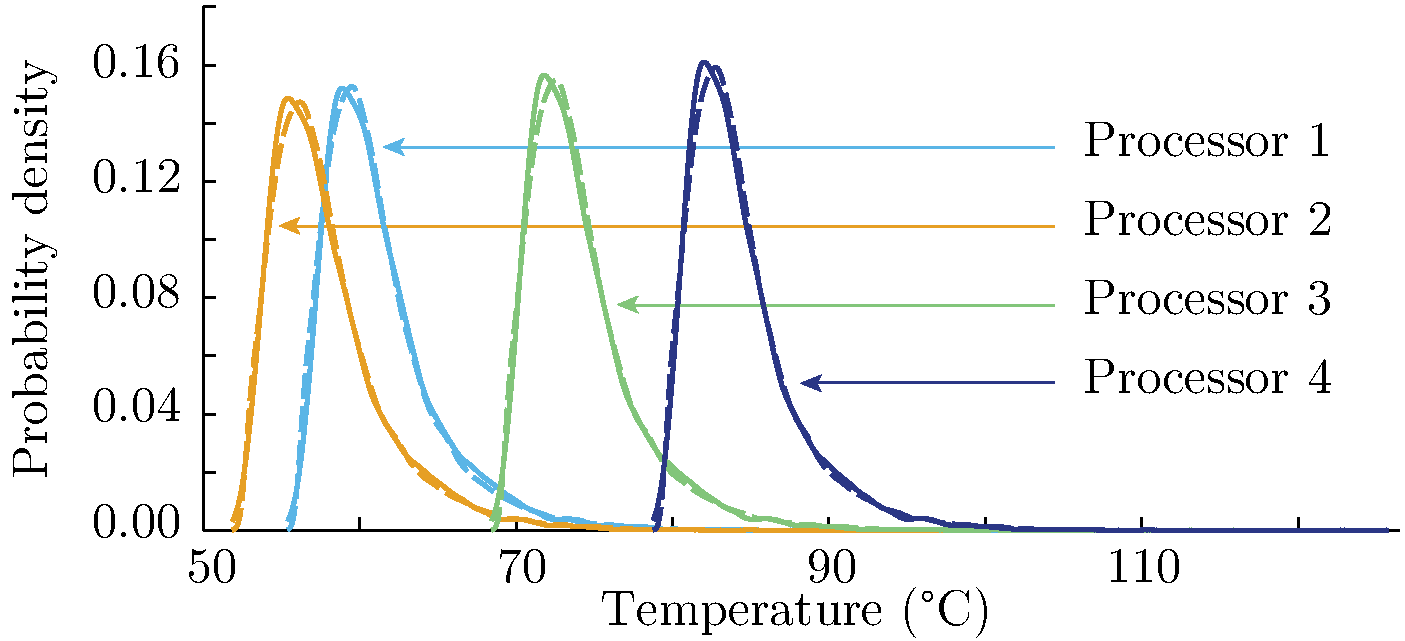
\includegraphics[width=1\ColumnWidth]{include/assets/experimental-results-pdf.pdf}
  \vspace{-2.0em}
  \caption{Probability density functions computed at time 50$\,\text{ms}$ using the proposed framework (the dashed lines) and MC sampling (the solid lines).}
  \flabel{experimental-results-pdf}
\end{figure}


\subsection{Accuracy \versus\ Spatial Correlations}
Let us have a look at the accuracy of the proposed framework with respect to different correlation patterns between the local random variables $\lLeff_i(\o)$ (recall \sref{illustrative-example}).
Specifically, we shall change the balance between the two correlation kernels shown in \eref{correlation-function}, \ie, the squared exponential $\fCorr_\SE$ and Ornstein-Uhlenbeck $\fCorr_\OU$ kernels.
The contributions of the kernels is controlled by $\eta$, which was set to its default value of $0.5$ in the experiment in \sref{er-polynomial-order} favoring no kernel.
Now we set it to the extreme values zero and one, which gives the full power either to $\fCorr_\SE$, when $\eta = 1$, or to $\fCorr_\OU$, when $\eta = 0$.

Guided by the above observations, we fix the polynomial order $\pcorder$ to four for the rest of the experiments and conclude that the error of our technique is bounded by less than $0.2\%$ for expectation and less than $2\%$ for variance and \pdf.
In addition, based \tref{accuracy-polynomial-order} together with theoretical estimates of the accuracy of MC sampling \cite{diaz-emparanza2002} and the experience from the literature \cite{xiu2010, maitre2010, shen2009, eldred2008}, we let the MC approach with the number of samples $\nsamples$ equal to $10^4$ be the etalon for the evaluation of the proposed framework.

\subsection{Computational Speed \versus\ Processing Elements}
Now we focus on the computational speed.
First, we vary the number of processing elements $\nprocs$, which, in its turn, affects the number of uncertain parameters $\vU(\o)$.
In these experiments, the number of time steps $\nsteps$ is constant and equal to $10^3$.
The results are given in \tref{speed-processing-elements} along with the number of the independent random variables $\vZ(\o)$, $\nvars$, left after the KL-based model order reduction procedure (see \sref{ie-uncertain-parameters}).
\begin{table}[h]
  \vspace{-0.5em}
  \centering
  \caption{Scaling with respect to the number of processing elements \textnormal{$\nprocs$}}
  \vspace{-0.5em}
  \begin{tabular*}{1\linewidth}{L{20pt}L{15pt}R{50pt}R{50pt}R{60pt}}
    \toprule
    $\nprocs$ & $\nvars$ & PC, seconds & MC, hours & Speedup, times \\
    \midrule
    \midrule
     2 & 2 & 0.28 & 30.98 & $3.99 \times 10^5$ \\
     4 & 3 & 0.30 & 31.04 & $3.73 \times 10^5$ \\
     8 & 4 & 0.59 & 31.06 & $1.88 \times 10^5$ \\
    16 & 5 & 1.37 & 38.97 & $1.03 \times 10^5$ \\
    32 & 6 & 6.78 & 40.27 & $2.14 \times 10^4$ \\
    \bottomrule
  \end{tabular*}
  \tlabel{speed-processing-elements}
  \vspace{-0.5em}
\end{table}


It can be seen that the correlations inherent to the fabrication process \cite{cheng2011} open a great possibility for model order reduction.
One can also observe a low slope of the execution time of the MC technique, which exhibits the well-known fact that the workload per one MC sample is independent of the number of stochastic dimensions \cite{maitre2010}.
However, even in high dimensions, the proposed framework significantly outperforms MC sampling. For instance, to quantify a power profile with $10^3$ steps of a system with 32 cores, the MC approach requires more than 40 hours whereas the proposed framework takes less than 10 seconds.

\subsection{Computational Speed: Time Spans}
Finally, we investigate the scaling properties of the proposed framework with respect to the duration of the considered time spans, which is directly proportional to the number of steps $\nsteps$ in the power and temperature profiles.
The results for a quad-core architecture are given in \tref{speed-time-spans}.
\begin{table}[h]
  \vspace{-0.5em}
  \caption{Scaling with respect to the number of steps \textnormal{$\nsteps$}}
  \vspace{-0.5em}
  \begin{tabular*}{1\linewidth}{cL{20pt}R{50pt}R{50pt}R{60pt}}
    \toprule
    & $\nsteps$ & PC, seconds & MC, hours & Speedup, times \\
    \midrule
    \midrule
    \multirow{5}{*}{\begin{sideways}$\eta = 0.0$\end{sideways}}%
    & $10$   & 00.00 & 00.00 & $0.00 \times 10^0$ \\
    & $10^2$ & 00.00 & 00.00 & $0.00 \times 10^0$ \\
    & $10^3$ & 00.00 & 00.00 & $0.00 \times 10^0$ \\
    & $10^4$ & 00.00 & 00.00 & $0.00 \times 10^0$ \\
    & $10^5$ & 00.00 & 00.00 & $0.00 \times 10^0$ \\
    \midrule
    \multirow{5}{*}{\begin{sideways}$\eta = 0.5$\end{sideways}}%
    & $10$   & 00.00 & 00.00 & $0.00 \times 10^0$ \\
    & $10^2$ & 00.00 & 00.00 & $0.00 \times 10^0$ \\
    & $10^3$ & 00.00 & 00.00 & $0.00 \times 10^0$ \\
    & $10^4$ & 00.00 & 00.00 & $0.00 \times 10^0$ \\
    & $10^5$ & 00.00 & 00.00 & $0.00 \times 10^0$ \\
    \midrule
    \multirow{5}{*}{\begin{sideways}$\eta = 1.0$\end{sideways}}%
    & $10$   & 00.00 & 00.00 & $0.00 \times 10^0$ \\
    & $10^2$ & 00.00 & 00.00 & $0.00 \times 10^0$ \\
    & $10^3$ & 00.00 & 00.00 & $0.00 \times 10^0$ \\
    & $10^4$ & 00.00 & 00.00 & $0.00 \times 10^0$ \\
    & $10^5$ & 00.00 & 00.00 & $0.00 \times 10^0$ \\
    \bottomrule
  \end{tabular*}
  \tlabel{speed-time-spans}
  \vspace{-0.5em}
\end{table}


Due to the long execution time demonstrated by the MC approach, its computational times for high values of $\nsteps$ are extrapolated based on a smaller number of samples, \ie, $\nsamples \ll 10^4$.
It can be seen that both methods scale linearly with $\nsteps$. However, the proposed framework shows a vastly superior performance.
